% This file is part of Combo Whist.
%
% Copyright 2007-2016 Joakim Nilsson
%
% This text is free software: you can redistribute it and/or modify
% it under the terms of the GNU General Public License as published by
% the Free Software Foundation, either version 3 of the License, or
% (at your option) any later version.
%
% This text is distributed in the hope that it will be useful,
% but WITHOUT ANY WARRANTY; without even the implied warranty of
% MERCHANTABILITY or FITNESS FOR A PARTICULAR PURPOSE.  See the
% GNU General Public License for more details.
%
% You should have received a copy of the GNU General Public License
% along with this text.  If not, see <http://www.gnu.org/licenses/>.

% Document class
\documentclass[a4paper]{article}

\usepackage[swedish]{babel}
% This file is part of Combo Whist.
%
% Copyright 2014-2016 Joakim Nilsson
%
% This text is free software: you can redistribute it and/or modify
% it under the terms of the GNU General Public License as published by
% the Free Software Foundation, either version 3 of the License, or
% (at your option) any later version.
%
% This text is distributed in the hope that it will be useful,
% but WITHOUT ANY WARRANTY; without even the implied warranty of
% MERCHANTABILITY or FITNESS FOR A PARTICULAR PURPOSE.  See the
% GNU General Public License for more details.
%
% You should have received a copy of the GNU General Public License
% along with this text.  If not, see <http://www.gnu.org/licenses/>.
% License notice
% Packages

\usepackage[utf8]{inputenc}
\usepackage[protrusion=true]{microtype} % More readable layout
\usepackage{graphicx}                   % For \rotatebox
\usepackage{tabularx}                   % For the X column specifier
\usepackage[pass]{geometry}             % For changing margins
\usepackage[labelfont=bf]{caption}      % Captions boldface
\usepackage{verbatim}
\usepackage{hyperref}

% Set-up reference style
\hypersetup{%
	pdfborderstyle={/S/U/W 1}
}

% Rotate text 90 degrees
\newcommand{\rotccw}[1] {%
	\rotatebox{90}{{#1}}
}

\newcommand{\standardBidItem}[6]{%
	\\ \hline
	\textit{#1} &
	#2 &
	#3 &
	#4 &
	#5 &
	#6
}

\newcommand{\specialBidItem}[4]{%
	\\ \hline
	\textit{#1} &
	#2 &
	\raggedright\textit{#3} &
	#4
}

\newcommand{\introPages}{%
	% Title
	\maketitle

	\vfill

	% Logo
	\begin{center}
		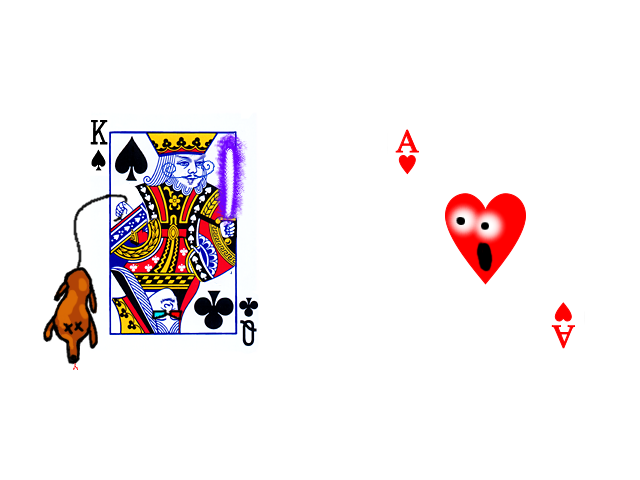
\includegraphics[width = \textwidth]{../logo.png}
	\end{center}

	\vfill

	% This file is part of Combo Whist.
%
% Copyright 2014-2016 Joakim Nilsson
%
% This text is free software: you can redistribute it and/or modify
% it under the terms of the GNU General Public License as published by
% the Free Software Foundation, either version 3 of the License, or
% (at your option) any later version.
%
% This text is distributed in the hope that it will be useful,
% but WITHOUT ANY WARRANTY; without even the implied warranty of
% MERCHANTABILITY or FITNESS FOR A PARTICULAR PURPOSE.  See the
% GNU General Public License for more details.
%
% You should have received a copy of the GNU General Public License
% along with this text.  If not, see <http://www.gnu.org/licenses/>.
% License notice

\begin{verbatim}
	Copyright 2007-2016 Joakim Nilsson

	This text is free software: you can redistribute it and/or modify
	it under the terms of the GNU General Public License as published by
	the Free Software Foundation, either version 3 of the License, or
	(at your option) any later version.

	This text is distributed in the hope that it will be useful,
	but WITHOUT ANY WARRANTY; without even the implied warranty of
	MERCHANTABILITY or FITNESS FOR A PARTICULAR PURPOSE.  See the
	GNU General Public License for more details.
\end{verbatim}
\verb|You should have received a copy of the GNU General Public License|\\
\verb|along with this text.  If not, see <|\url{http://www.gnu.org/licenses/}\verb|>.|


	\thispagestyle{empty}
	\pagebreak

	% Table of contents and list of tables
	\microtypesetup{protrusion=false} % No protrusion for table of contents
	\setcounter{tocdepth}{3}
	\tableofcontents
	\listoftables
	\microtypesetup{protrusion=true} % Re-enable protrusion
	\thispagestyle{empty}
	\pagebreak
}


% Title
\title{Kombinations-Whist}
\author{Av Joakim Nilsson}
\date{Utvecklarversion (baserad på version 1.1.1-sv) --- \today}

% Document
\begin{document}
	\introPages

	\section{Översikt}{%
		Kombinations-Whist är ett kortspel som bygger på sticktagande och är, som namnet antyder, en variant av Whist. Kombinations-Whists huvudsakliga utmärkande drag är dess varierade utbud av möjliga strategier med acceptabelt simpla regler. (Det måste dock erkännas att regelboken trots det är någorlunda lång.) Möjligheten att spela enligt många varierade strategier tar bort en substantiell mängd slump som vanligtvis finnes i andra Whist-spel utan att att göra spelet alltför komplicerat. Detta gör Kombinations-Whist till ett spel som är kul att spela både för erfarna spelare såväl som för nybörjare.

		\paragraph{Antal spelare:}
		4 är att föredra, men 3 till $\infty$ går också bra med vissa regeländringar.

		\paragraph{Vad som behövs för att spela:}
		En standard-kortlek med 52 kort samt penna och papper.

		\paragraph{Kortens värde:}
		Från högst till lägst: E, K, D, Kn, 10, 9, 8, 7, 6, 5, 4, 3, 2
	}

	\section{Hur man spelar}{%
		\subsection{Förberedelser}{%
			Gör en kolonn för varje spelare på pappret. Detta för att hålla koll på poängställningen samt lite annan information om spelet. Efter att pappret är förberett, slumpa då fram vem som blir giv.
		}

		\subsection{Given}{%
			Det finns två huvudsakliga delar av en giv. Den första är \emph{budgivningen} och den andra är \emph{spelet}. Eftersom det borde bli lättare att förstå dessa två delar i omvänd ordning beskrivs spelet före budgivningen.

			En giv börjar med att given delar ut 13 kort till varje spelare (eller 17 om det bara finns 3 spelare, i vilket fall $\clubsuit 2$ tas bort ur leken). Därefter börjar budgivningen och när den är avklarad börjar spelet.

			Efter spelet noteras spelarnas poäng och en ny giv börjar där spelaren till vänster om den föregående given blir ny giv.

			\subsubsection{Spelet}{%
				Spelet spelas likt de flesta Whist-varianter. Spelaren till höger om \emph{spelföraren}\footnote{Termen ``spelförare'' förklaras i stycket \textit{\nameref{sec:bidding}}.} börjar med att spela ut en kort. Sen blir det spelaren till höger om denne som spelar ut nästa kort som dessutom måste följa färg. Därefter spelar näste spelare (till vänster om föregående) ut ännu ett kort som också måste följa det första kortets färg och så vidare till det att alla spelare har spelat ut ett kort vardera.

				Om en spelare har slut kort i den först utspelade färgen får denne saka valfritt kort eller spela en trumf. Till skillnad från många Whist-varianter finns inget trumftvång.

				Den spelare som spelade det högsta kortet i den först utspelade färgen tar hem \emph{sticket} (det vill säga, tar alla utspelade kort och lägger dem med bildsidan ned på bordet) såvida ingen har spelat ut en trumf. Om så skulle vara fallet är det den spelare som har spelat ut den högsta trumfen som tar hem sticket.

				Den spelare som tog hem det senaste sticket spelar ut först i nästa.
			}

			\subsubsection{Budgivningen}{\label{sec:bidding}
				I Kombimations-Whist bjuder man med \emph{kombinations-bud}. Ett kombinations-bud består av precis ett standardbud och en valfri mängd (inklusive noll) specialbud. Buden har särskilda regler som förknippas med dem, vilka appliceras under spelet och poängberäkningen. Om det är oklart \emph{när} en händelse som inträffar på grund av ett bud ska ske så går standardbudens händelser före specialbudens.

				Spelarna bjuder medsols och spelaren till vänster om given börjar. En spelar kan antingen passa eller bjuda ett kombinations-bud som är värt mer än föregående kombinations-bud (som vi, från och med nu, helt enkelt kommer att kalla bud). Om en spelare passar är denne ute ur budgivningen och får därför inte göra några nya bud förrän nästa giv. Om alla spelare passar blir det omgiv där samme giv ger igen.

				Ett buds värde definieras som det kombinerade värdet av standard- och specialbudet som det består av. Det föreslås att en tidsgräns på 20 sekunder sätts mellan varje bud och 1 minut före det första budet. För nybörjare är dock längre eller inga tidsgränser rekommenderade. Om en spelare inte har lagt ett bud inom den givna tiden så passar denne automatiskt. Budgivningen fortsätter fram till att alla spelare förutom en har passat. Den spelaren blir spelförare och spelet börjar.

				De standardbud och specialbud som finns att tillgå finns listade i Tabellerna~\ref{tab:standardBids}~respektive~\ref{tab:specialBids}. Antalet stick att ta hem för att ett bud ska gå hem finnes i standardbudstabellens ``Stick''-kolonn. Ett specialbud kan inte kombineras med ett annat bud som finns listade i ``Inkompatibilitet''-kolonnen. Notera att det finns en skillnad mellan värde och poäng. Värde är budets värde (Rätt gissat!) och poäng är antalet poäng som spelföraren får om dennes bud går hem.

				De stanardbud som är markerade med en asterisk (*) har andra regler i fallet när bara 3 spelare deltar i spelet. Dessa bud finns listade i Tabell~\ref{tab:standardBids3}.
			}

			\subsubsection{Poängberäkningen}{%
				Efter att spelet är klart så får spelföraren ett antal poäng baserat på vilket kombinations-bud som bjöds och huruvida detta bud gick hem. Om budet gick hem får spelföraren det antal poäng som specificeras ``Poäng''-kolonnen för standardbudet. Om budet inte gick hem så förlorar spelföraren 2 poäng. En spelare kan anta en negativ poängsumma. Om en spelare antar en poängsumma lägre än -5, så tillåts denne inte längre att bjuda i budgivningar. Hen får dock 1 gratispoäng när den given är klar (även om ingen bjuder och det blir omgiv).
			}

			\subsubsection{Vem som vinner}{%
				Den som först uppnår \emph{vinstsumman} vinner. Vinstsumman börjar på 13, men minskar med 1 varje gång alla spelare har varit giv en gång vardera. En spelare kan endast vinna genom att ett bud går hem och kan därför inte vinna enbart därför att vinstsumman just minskade. En spelare kan inte heller vinna om denne inte har enskilt flest poäng.
			}
		}
	}

	\section{Övrigt}{%
		\subsection{Regler för fler än 4 spelare}{%
			Om fler är 4 spelare deltar i spelet så får alla utom 4 sitta ut (avstå att delta) i varje giv. De spelare som sitter ut är de som sitter närmast till höger om given.
			
			% Changes for 3 players table
			\begin{table}
	\begin{center}
		\footnotesize {
			\begin{tabular}{ p{2.0cm} | p{1.0cm} }
					Name & Books
					\\ \hline
					Trump & min 7 \\ \hline
					Grill & min 7 \\ \hline
					Spades & min 7 \\ \hline
					Play & min 7 \\ \hline
					Trick play & min 7 \\ \hline
					Max trump & min 9 \\ \hline
					Round trump & min 7 \\ \hline
					Master trump & min 7
			\end{tabular}
		}
	\end{center}
	\caption{Standard bids, modified to suit 3 players}
	\label{tab:standardBids3}
\end{table}

		}
		
		\subsection{Prat}{%
			En viss mängd av prat tillåts i Kombinations-Whist, men spelarna tillåts inte ge \emph{några som helst} ledtrådar om vad de har för kort.
		}
		
		\subsection{Fusk}{%
			En spelare som avsiktligen fuskar i Kombinations-Whist får aldrig mer spela spelet eftersom denne uppenbarligen inte respekterar spelets prakt.
		}

		\subsection{Versionsnummer}{%
			Kombinations-Whists versionsformat specifieras som följer:

			\begin{verbatim}
				<huvudversion> . <underordnad version> . <revision> - <språk>
			\end{verbatim}

			Huvudversionen ökar enbart när omvälvande ändringar görs i spelet. Det är osannolikt att detta nånsin kommer att hända.

			Den underordnade versionen ökar när signifikanta ändringar görs i reglerna. Till exempel skulle nya bud eller att bud tas bort motivera en ny underordnad version.

			Revisionen ökar när små ändringar görs till parametrar i spelet, såsom en ändring i ett buds värde.
		}
	}

	% Bid tables
	\pagebreak
	\newgeometry{left=1cm, right=1cm, top=1cm}
	% This file is part of Combo Whist.
%
% Copyright 2007-2016 Joakim Nilsson
%
% This text is free software: you can redistribute it and/or modify
% it under the terms of the GNU General Public License as published by
% the Free Software Foundation, either version 3 of the License, or
% (at your option) any later version.
%
% This text is distributed in the hope that it will be useful,
% but WITHOUT ANY WARRANTY; without even the implied warranty of
% MERCHANTABILITY or FITNESS FOR A PARTICULAR PURPOSE.  See the
% GNU General Public License for more details.
%
% You should have received a copy of the GNU General Public License
% along with this text.  If not, see <http://www.gnu.org/licenses/>.

\begin{table}
	\caption{Standardbud}\label{tab:standardBids}
	\begin{center}
		\begin{tabularx}{\textwidth}{lcccc|X}
				\textbf{Namn} &
				\rotccw{\textbf{Värde}} &
				\rotccw{\textbf{Poäng}} &
				\rotccw{\textbf{Trumf}} &
				\rotccw{\textbf{Stick}} &
				\textbf{Tilläggsregler}
				\\[-3ex]

				\standardBidItem%
				{Dumskipp}
				{$0$}
				{$1$}
				{nej}
				{varierar}
				{%
					Spelföraren får inte ta hem flest stick --- inte ens om nån annan spelare har tagit hem lika många stick.
				}

				\standardBidItem%
				{Ungefär}
				{$1$}
				{$1$}
				{nej}
				{varierar}
				{%
					Före spelets början gissar spelföraren på två möjliga mängder stick denne kommer att ta hem. Hen måste ta hem en av de två möjliga mängderna som gissades.
				}

				\standardBidItem%
				{Trumf*}
				{$1$}
				{$1$}
				{ja}
				{min 5}
				{%
					Spelföraren bestämmer trumffärg.
				}

				\standardBidItem%
				{Grill*}
				{$1$}
				{$2$}
				{ja}
				{min 5}
				{%
					Spelföraren börjar med att bestämma trumffärg. Denna trumffärg gäller bara första sticket. Därefter blir den färg som spelades ut i föregångde stick ny trumffärg och så fortsätter det till spelets slut.
				}
				
				\standardBidItem%
				{Spader*}
				{$2$}
				{$1$}
				{ja}
				{min 5}
				{%
					Trumffärgen är spader.
				}

				\standardBidItem%
				{Spel*}
				{$2$}
				{$2$}
				{nej}
				{min 5}
				{%
					---
				}

				\standardBidItem%
				{Skipp*}
				{$3$}
				{$2$}
				{nej}
				{varierar}
				{%
					Spelföraren måste ta hem färst stick. Om ingen tar hem färre stick än spelföraren går budet hem.
				}

				\standardBidItem%
				{Exakt}
				{$3$}
				{$2$}
				{nej}
				{varierar}
				{%
					Före spelets början gissar spelföraren på en möjlig mängd stick denne kommer att ta hem. Hen måste ta hem den mängd som gissades.
				}

				\standardBidItem%
				{Maxtrumf*}
				{$3$}
				{$3$}
				{ja}
				{min 7}
				{%
					Spelföraren väljer trumffärg.
				}

				\standardBidItem%
				{Smygtrumf*}
				{$3$}
				{$3$}
				{ja}
				{min 5}
				{%
					Spelföraren väljer trumffärg. Hen får dock inte välja en trumffärg som hen har flest kort i.
				}

				\standardBidItem%
				{Mästarspel}
				{$4$}
				{$3$}
				{nej}
				{varierar}
				{%
					Spelföraren måste ta hem flest stick. Om denna tar hem lika många som nån annan spelare så går budet inte hem.
				}

				\standardBidItem%
				{Noll}
				{$4$}
				{$4$}
				{nej}
				{0}
				{%
					---
				}

				\standardBidItem%
				{Mästartrumf*}
				{$6$}
				{$6$}
				{ja}
				{min 5}
				{%
					Spelaren till vänster om spelföraren bestämmer trumffärg, men först får de andra icke-spelförarna säga vilken trumffärg de föredrar och hur mycket de föredrar denna på en skala från $1$ till $10$ (utan motivering).
				}

				\standardBidItem%
				{Obesudlat Mästarspel}
				{$9$}
				{X}
				{nej}
				{alla}
				{%
					Om budet går hem får spelföraren lika många poäng som kombinations-budets värde. Skulle dessutom kombinations-budets värde vara $13$ eller högre vinner spelföraren spelet omedelbart oavsett poängställning. När detta inträffar erhåller dessutom spelföraren rätten att titulera sig \emph{Obesudlad Mästare av Kombinations-Whist} under resten av sitt liv. Om spelföraren tar hem färre än hälften av sticken förlorar denne dubbelt som många poäng som hen annars skulle ha gjort.
				}
		\end{tabularx}
	\end{center}
\end{table}

	% This file is part of Combo Whist.
%
% Copyright 2007-2016 Joakim Nilsson
%
% This text is free software: you can redistribute it and/or modify
% it under the terms of the GNU General Public License as published by
% the Free Software Foundation, either version 3 of the License, or
% (at your option) any later version.
%
% This text is distributed in the hope that it will be useful,
% but WITHOUT ANY WARRANTY; without even the implied warranty of
% MERCHANTABILITY or FITNESS FOR A PARTICULAR PURPOSE.  See the
% GNU General Public License for more details.
%
% You should have received a copy of the GNU General Public License
% along with this text.  If not, see <http://www.gnu.org/licenses/>.

\newcommand{\nonTrump}{\textnormal{non-trump bids}}

\begin{table}
	\caption{Special bids}\label{tab:specialBids}
	\begin{center}
		\begin{tabularx}{\textwidth}{lS[table-number-alignment=center]p{3cm}|X}
			\textbf{Name} &
			\textbf{Worth} &
			\textbf{Incompatibility} &
			\textbf{Additional rules}
			\\[-3ex]

			\specialBidItem%
			{Sloth}
			{-3}
			{---}
			{%
				For the tricks in which the declarer doesn't lead, the declarer plays their card last.
			}

			\specialBidItem%
			{Triumph Trump}
			{-3}
			{---}
			{%
				The declarer selects any card before the game begins. This card becomes the \emph{triumph trump}. The declarer decides who takes a trick containing the triumph trump when this trick is brough home. A triumph trump does \emph{not} change suit to the trumph suit, but retains its old suit.
			}

			\specialBidItem%
			{Potential}
			{-2}
			{---}
			{%
				If this bid is completed it is marked by a P, a \emph{potential}, in the declarer's column. A player can only have one P in their column.
			}

			\specialBidItem%
			{Start}
			{-2}
			{---}
			{%
				The declarer leads the first trick.
			}

			\specialBidItem%
			{Switcharoo}
			{-1}
			{---}
			{%
				Before the game starts, all players send 3 cards in a direction the declarer chooses (to the right, to the left or across).
			}

			\specialBidItem%
			{Iron}
			{-1}
			{---}
			{%
				The aces now rank the lowest.
			}

			\specialBidItem%
			{Greed}
			{0}
			{---}
			{%
				At the end of the game 1 trick is added to or subtracted from the declarer's stick count so that it doesn't benefit them. If the bid is completed, the declarer scores 1 extra point.
			}

			\specialBidItem%
			{Finishing Dog}
			{1}
			{Zero}
			{%
				The declarer must not bring home the last trick.
			}

			\specialBidItem%
			{Atelier}
			{1}
			{Open Hand}
			{%
				The declarer chooses 4 cards that they put in \emph{the atelier}. These cards must be shown to all players during the game. As soon as the atelier no longer consists of 4 cards, the declarer must add a card to it provided they have cards in their hand.
			}

			\specialBidItem%
			{Open Trump}
			{1}
			{\nonTrump, Grill, Open Hand}
			{%
				The declarer must play with open trump cards. That is, all of the declarer’s trump cards must be shown to all players during the game. If combined with \emph{Atelier}, the atelier must not contain any trump cards.
			}

			\specialBidItem%
			{Lock}
			{2}
			{Zero}
			{%
				The declarer must not bring home any of the first 3 tricks.
			}

			\specialBidItem%
			{Punishment}
			{2}
			{---}
			{%
				If the declarer does not complete their bid, 2 extra points are subtracted from their score.
			}

			\specialBidItem%
			{Extended Bid}
			{2}
			{---}
			{%
				This bid may only be bid if the declarer has a P in their column (which can be aquired by completing \emph{Potential}). When this bid is part of the highest combo bid, the P that the declarer aquired P is crossed out.
			}

			\specialBidItem%
			{Master's Switcharoo}
			{3}
			{\nonTrump, Grill}
			{%
				Before the game starts, all players but the declarer sends 4 cards to the player to the right (skipping the declarer). If \emph{Switcharoo} has been bid, the \emph{Switcharoo}-cards are sent before the \emph{Master's Switcharoo}-cards.
			}

			\specialBidItem%
			{Open Hand}
			{3}
			{Atelier, Open Trump}
			{%
				The declarer must play with an open hand. That is, all of the thier cards must be shown to all players during the game.
			}
		\end{tabularx}
	\end{center}
\end{table}

\end{document}
